
\chapter{Clustering}
\label{ch:Clustering}

Clustering algorithms divide a dataset into several disjoint subsets. All elements in such
a subset share common features like, for example, spatial proximity.
Clustering is used as a stand-alone tool to get insight into the distribution
of a data set or as a preprocessing step for other algorithms operating on the
detected clusters. The former is used to determine stop criteria as described
in Section \ref{sec:TermConditions} and the latter is used in our fitness deterioration
algorithm to improve its accuracy.

A cluster extension (see Definition \ref{def:cluster_extension}) 
may be seen as an approximation of the basin of attraction,
moreover the distribution of individuals which were flooded to the basins provides 
additional useful information about its shape. 
The clustering algorithm may be used to detect the set of individuals which
belongs to the same basin of attraction. 
The CSFD provides the information about detected
sets (basins of attraction) in the form of a proper representation of 
cluster extensions which are just a convenient way to describe basins of attraction 
(e.g the center point, the radius of the set, covariance matrix etc.). 

\section{OPTICS}
\label{sec:OPTICS}

We have choosen density-base clustering algorihtm called \textit{OPTICS:
Ordering Points To Identify the Clustering Structure} \cite{optics}. 
Density-base clustering generally needs the data which is the subset
or the multiset of objects (points) which belong to a finite dimensional
vector metric space $V$.
Clusters are regarded as subsets in which the objects are 
dense and which are separated by regions of low object density.
These subsets may have an arbitrary shape and the points inside a region
may be arbitrarily distributed.

\textit{OPTICS} is an extendsion to a well-known density clustering algorithm
called \textit{DBSCAN} \cite{dbscan}. The basic idea for \textit{DBSCAN} is that
for each point of a cluster the neighborhood of a given radius $\epsilon$ has to contain
at least a minimum number of points $minPts$. Figure
\ref{fig:clusters} shows the result of \textit{OPTICS} clustering for a sample set of points.

In particular each object $q$ of the cluster $C$ 
has to be surrounded by the neighborhood $N_{\epsilon}(q) \subset V$
of a given radius $\epsilon$ that contains at least $minPts$ other objects.
The formal definition for this notion is as follows:

\begin{figure}
  \centering
  \fbox{
    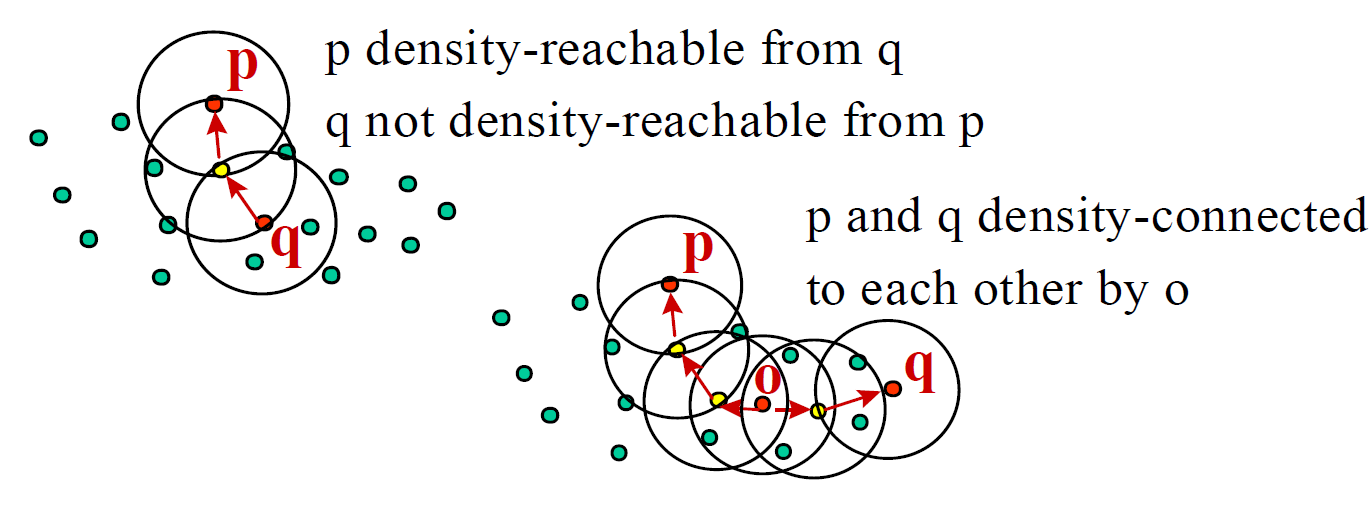
\includegraphics[scale=0.2]{densityReachability.png}
  }
  \caption{Density-reachability and connectivity}
  \label{fig:densityReach}
\end{figure}

\vspace{5pt}
\begin{definition}
\label{def:directly-den-reach}
An object $p \in P$ is \textit{directly
density-reachable} from an object $q\in P $ 
with respect to the parameters 
$\epsilon \in \mathbb{R}_+$, $minPts \in \mathbb{N}$ 
in a set or multiset of data $P$ if:
\begin{itemize}
  \item $p \in N_{\epsilon}(q)$, 
  \item $Card(N_{\epsilon}(q) \cap P) \geq minPts$.
\end{itemize}
\end{definition}
\vspace{5pt}

The condition $Card(N_{\epsilon}(q)  \cap P) \geq minPts$ is called the 
\textit{core object condition}. 
If this condition holds for an object $q$, then we call
$q$ a \textit{core object}. Only from core objects, other objects can be
directly density-reachable.

\vspace{5pt}
\begin{definition}
\label{def:den-reach}
An object $p$ is \textit{density-reachable} from an object $q$ 
with respect to the parameters 
$\epsilon \in \mathbb{R}_+$,
in the set or multiset of objects $P$ if there is a chain of objects $p_1,
\ldots, p_n, p_1=q,p_n=p$ such that $p_i \in P$ and $p_{i+1}$ is directly
density-reachable from $p_i$ for $i = 1, \ldots, n-1$ 
with respect to $\epsilon$ and $minPts$.
\end{definition}
\vspace{5pt}

The density-reachability relation is not symmetric in general in $P$. 
Only core objects can be mutually density-reachable.

\vspace{5pt}
\begin{definition}
\label{def:den-connect}
An object $p$ is \textit{density-connected} to an object $q$ 
with respect to $\epsilon$ and
$minPts$ in the set or multiset of objects $P$ if there is an object $o \in P$ 
such that both $p$ and $q$ are density-reachable from $o$ 
with respect to $\epsilon$ and $minPts$ in $P$.
\end{definition}
\vspace{5pt}

Both phenomena are illustrated by Figure \ref{fig:densityReach}.
A density-based \textit{cluster} is now defined as a multiset of
density-connected objects which is maximal with respect to density-reachability 
and the \textit{noise} is the 
set of objects not contained in any cluster.

\vspace{5pt}
\begin{definition}
\label{def:cluster-noise}
Let $P$ be a set or multiset of objects. A cluster $C$ 
with respect to $\epsilon$ and $minPts$ in
$P$ is a non-empty subset of $P$ satisfying the following conditions:
\begin{itemize}
  \item Maximality: $\forall p,q \in P$: if $p \in C$ and $q$ is
  density-reachable from $p$ wrt. $\epsilon$ and $minPts$, then also $q \in C$.
  \item Connectivity: $\forall p,q \in C$: $p$ is density-connected to $q$ wrt.
  $\epsilon$ and $minPts$ in $P$.
\end{itemize}
Every object not contained in any cluster is \textit{noise}.
\end{definition} 
\vspace{5pt}



\textit{OPTICS} works like \textit{DBSCAN} but for an infinite number of
distance paramters $\epsilon_i$ which are smaller than a \textit{generating distance}
$\epsilon$. The only difference is that we do not assing cluster memberships.
Instead, we store the \textit{order} in which the objects are processed (the
main priniple is that we always have to select an object which is
density-reachable with respect to the lowest $\epsilon$ value to guarantee that
clusters with higher density are finished first) and the information which would
be used by \textit{DBSCAN} algorithm to assing cluster memberships. This
information consists of only two values for each object: \textit{core-distance}
and \textit{reachability-distance}.

\vspace{5pt}
\begin{definition}
\label{def:core-distance}
Let $p \in P$, let $\epsilon$ be a distance
value, let $N_{\epsilon}(p)$ be the $\epsilon$-neighborhood of $p$, 
let $minPts$ be a natural number and let $minPts-distance(p)$ be the distance
from $p$ to its $minPts$ neighbor. Then, the \textit{core-distance} of $p$ is
defined as:
$$
\text{core-distance}_{\epsilon,minPts}(p)= \left\{ \begin{array}{l}
\text{UNDEFINED, if } Card(N_{\epsilon}(p)) < minPts\\ 
\text{minPts-distance(p), otherwise} 
\end{array} \right
$$ 
\end{definition}
\vspace{5pt}

\vspace{5pt}
\begin{definition}
\label{def:reach-dist}
Let $p,o \in P$ let $N_{\epsilon}(o)$ be the
$\epsilon$-neighborhood of $o$, and let $minPts$ be a natural number.
Then, the \textit{reachability-distance} of $p$ with respect to $o$ is defined as:
$$
\text{reachability-distance}_{\epsilon,minPts}(p,o)= \left\{ \begin{array}{l}
\text{UNDEFINED, if } |N_{\epsilon}(o)| < minPts\\ 
\text{max(core-distance(o), distance(o,p)), otherwise} 
\end{array} \right
$$ 
\end{definition}
\vspace{5pt}

An advantage of cluster-ordering a data set compared to other clustering methods
is that the ordering (which might be visualized by \textit{reachability-plot} of
ordered points) is rather insensitive to the input parameters of the method i.e.
the \textit{generating distance} $\epsilon$ and the value for $minPts$. Roughly
speaking, the values have just to be \textit{large} enough to yield a good
result. The concrete values are not crucial because there is a broad range of
possible values for which we always can see the clustering structure of a data
set when looking at the corresponding \textit{reachability-plot}.
Figure \ref{fig:reachDist} shows reachablity plot for various \textit{generating
distances} ($\epsilon$) which might be seen as an empirical verification of the
last argument.

The next chapter describes how \textit{OPTICS ordering} properties are used
to prevent degradation of areas which have not been explored during the course
of the algorithm. 

\begin{figure}
  \centering
  \fbox{
    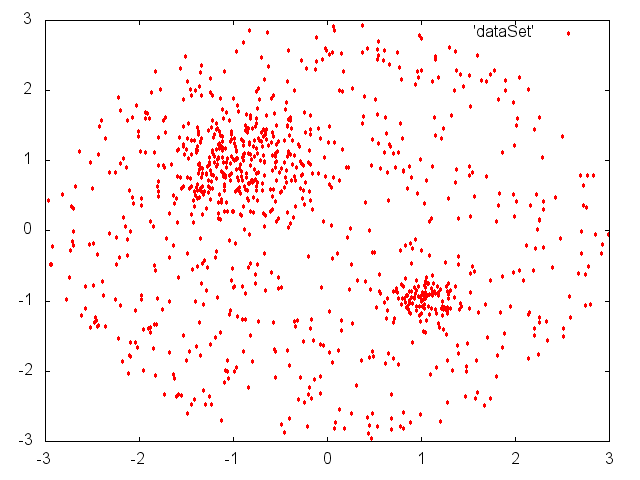
\includegraphics[scale=0.4]{dataSet.png}
  }
  \fbox{
    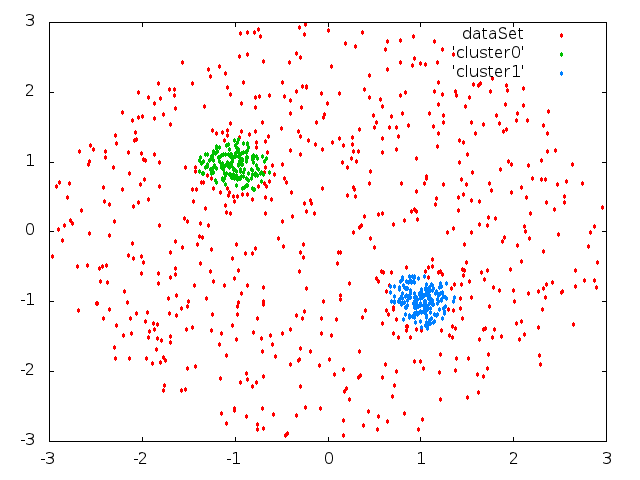
\includegraphics[scale=0.4]{clusters.png}
  }
  \caption{Visualization of the DBSCAN algorithm applied to OPTICS ordering
  of simple 2-dimensional data set which consists of 1000 points. OPTICS
  paramters: $minPts=20, \epsilon=1.2$, the two clusters was found using DBSCAN
  paramters: $\epsilon'=0.2$ (see \cite{optics} to fully understand the
  meaning of the parameters)}
  \label{fig:clusters}
\end{figure}


\begin{figure}
  \centering
  \fbox{
    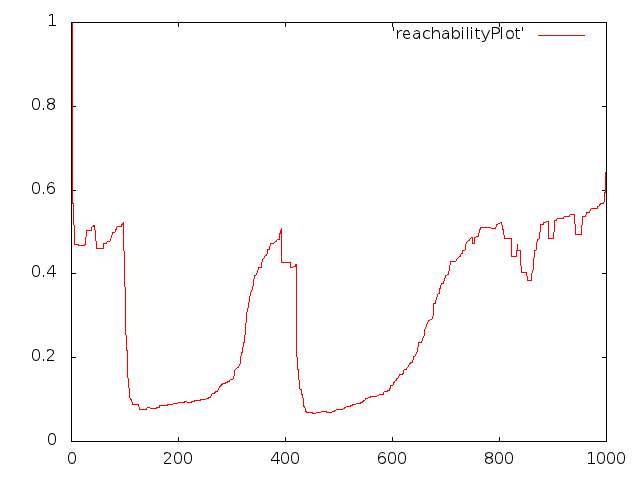
\includegraphics[scale=0.4]{reachability/1_5_20.png}
  }
  \fbox{
    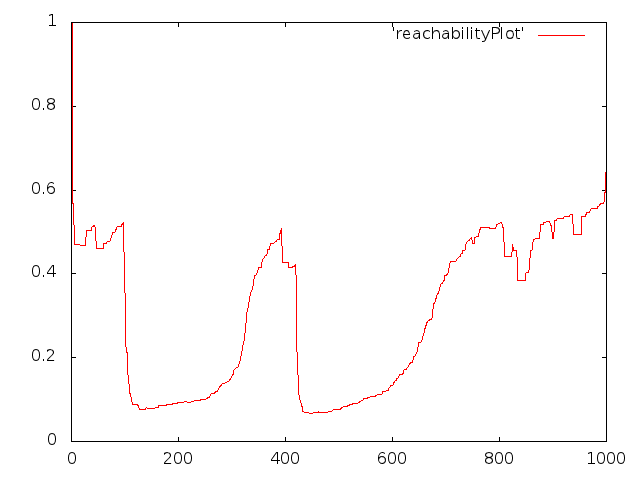
\includegraphics[scale=0.4]{reachability/1_0_20.png}
  }
  \fbox{
    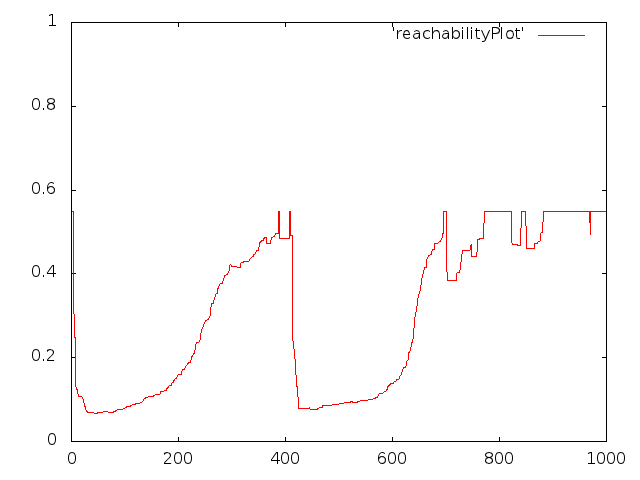
\includegraphics[scale=0.4]{reachability/0_5_20.png}
  }
  \caption{Reachability plot for data set presented on figure 3.1. Optics
  paramters (minPts, $\epsilon$) are: (20, 1.5), (20, 1.0), (20, 0.5)
  respectively. The two cavities which are visible in each plot depict the two
  of the clusters on figure 3.1. This proves that there is a large range of
  values for $\epsilon$ (\textit{generating distance}) for which the appearance
  of the reachability plot will not change significantly. (the flat shape of function from the last plot
  results from the fact that we truncate the reachability-distance to the 
  generating distance $\epsilon$, when the former is greater than the latter)}
  \label{fig:reachDist}
\end{figure}

